\documentclass[11pt, oneside]{article}   	% use "amsart" instead of "article" for AMSLaTeX format
\usepackage{geometry}                		% See geometry.pdf to learn the layout options. There are lots.
\geometry{letterpaper}                   		% ... or a4paper or a5paper or ... 
%\geometry{landscape}                		% Activate for rotated page geometry
%\usepackage[parfill]{parskip}    		% Activate to begin paragraphs with an empty line rather than an indent
\usepackage{graphicx}				% Use pdf, png, jpg, or eps§ with pdflatex; use eps in DVI mode
								% TeX will automatically convert eps --> pdf in pdflatex		
\usepackage{amssymb}
\usepackage{color}

%SetFonts

%SetFonts


\title{Conceptual devel. of the answer to running ChaNGa on Comet}
\author{johnny}
%\date{}							% Activate to display a given date or no date

\begin{document}
\maketitle
%\section{}
%\subsection{}

\begin{center}
TABLE OF CONTENTS
\end{center}
\bigskip

\begin{tabbing}
xxxxxxxxxxxxxxxxxxxxxxxxxxxxxxxxxxxxxxxxxxxx    \= xxxxxxxxxxxxxxx   \= xxxxxxxxxx   \kill
\\
Introduction: long background of comet    \>work with Tom   \>1 - 3     \\
    \>   \>   \\
history of commands: tom's office \& mahidhar   \>    \> 7 - 16    \\
    \>   \>   \\
    cube300.qsub\>   \>   \\
    \>   \>   \\
    \>   \>   \\
    \>   \>   \\
    \>   \>   \\

\end{tabbing}


\newpage

\begin{center}
\textsc{Introduction}
\end{center}

\begin{enumerate}
  \item Background
  \bigskip
  
	  \begin{enumerate}
	  \item Starting from scratch: it was easy and clearly documented how to logon to the Comet site.
	  \bigskip	
	 
	  \item Also clear to NOT run simulations in the home directoty
	  \bigskip	
	 
	  \item {\color{red}UNCLEAR} How to get ChaNGa and charmrun on to Comet.
	  
	  a) Getting those programs on the laptop was achieved without using Git.
	  
	  b) After the first 20-minute session with Tom that got ChaNGa finally running on EBTH it was clear the Git needed to be understood.
	  \bigskip	
	 
	  \item Umali's book on Git was a great help.
	  \bigskip	
	 
	  \item Mahidhar indicate that Git was on Comet, but I could not easily figure out how to find it.  Should more precisely document that answer.  Basically, it took some poking around on Comet to find ``bin.''  A good HW assignment.
	  \bigskip	
	 
	  \item {\color{blue}Git clone}.  Umali's book helped to figure out the vagaries of Git jargon that confuse the process in many other sources. Examples are the word ``repository,'' ``cloning,'' etc.
	  \bigskip	
	 
	  \item After practicing with Umali's stuff -- just a little, then at the command line it was possible to try some Git clones in Comet.
	  \bigskip	
	 
	  \item Some recommended command line stuff was slightly wrong.  Cannot remember, how I figured out how to enter the correct 
	  
	  git clone \_\_
	  
	  \bigskip	
	 
	  \item Somehow the git clone commands worked and changa and charm ``repositories'' -- really just directories.
	  \bigskip	
	 
	  \item After that success, Comet languished for awhile because I was trying to make some progress on ICIng which involved finding a good way to learn Python.
	  \bigskip	
	 
	  \item No Starch Press, Crash Python Course has some problems, but did the job and I wrote a couple of Python programs
	  \bigskip	
	 
	  \item I tried to build ChaNGa and charmrun about the last week of Feb. 2016 and got a make error.
	  \bigskip	
	 
	  \item I sent the ``make'' error to Mahidhar and got a great response. 
	  
	  a. He started working on the problem in earnest, and I seemed to be able to help a bit.  The details about this interaction would be great.
	  
	  b. He got ChaNGa ... so that was great then he wanted to try to run the simulation.
	  
	  c. I copied testcosmo and it's relevant parts to Comet.
	  
	  d. I also copied ChaNGa and charmrun to that folder.
	  

	  e. I ran into Tom and indicated that I was making great progress on Comet.
	  
	  f. The next day, Friday 2016-02-03  I saw Tom and he mentioned {\color{red}verbs} but I was pretty confused, so he invited me to his office.  Just before going to Tom's office I looked for the testcosmo-comet folder, and it was gone.

	  g.  Mahidhar transferred that folder to ``Oasis'' for running, but I didn't know that.
	  
	  h. When I looked at Mahidhar's code it was clear that he was trying to use the {\color{red}verb} implementation.   I spent some time reading about InfiniBand -- cool system for allowing applications to talk to each toher without having to go through the OS.  I suggested to Mahidhar, that he try the straight MPI implementation -- which kind of ruins the point of  charm, but should be a great first steap.
	  \bigskip	
	 
	  \item Tom almost got ChaNGa running on Comet, and then the next day Mahidhar got it running.
	  \bigskip	
	 
	  \item 
	  \bigskip	
	 
	 \end{enumerate}
  
  \bigskip

  \item
  \bigskip

  \bigskip
\end{enumerate}

\newpage

\begin{center}
\textsc{Put together a plan for what needs documentation}
\end{center}

\begin{enumerate}
  \item 
  \bigskip
  
In Tom's office he did the following which I need to review and document from the history command.
  \bigskip

  \item 
  \bigskip

  He copied a qsub - sbatch file from {\color{red}his} Comet folders!
  \bigskip
  \item
  \bigskip

{\color{blue} Assignment: figure out the difference between qsub and sbatch}
Thought that they were synonyms, but seems not.  First stab, maybe qsub is the command line statement and sbatch is part of the script?  
  \bigskip
  \item
  \bigskip
  
Tom mentioned the ``option'' of the command for running a build that uses the
{\color{red}j} -- It was clear that this option of the build command employed more {\color{blue}either cores or processors -- another potential assignment} because I could see it running faster compared to what I had just done on my own.
  \bigskip
  \item
  \bigskip

So the ``j'' option is clear on the {\color{red}operational} level.  
  \bigskip
  \item
  \bigskip
  
  There are many command line statements that both Tom and Mahidhar were using that will need lots of study.
  \bigskip
  \item
  \bigskip
  
  The Conclusion in Tom's office was that my version of ChaNGa was way too old.
  \bigskip
  \item
  \bigskip
  
  Tom was able to see that Mahidhar had tried to implement the ibverbs version from the history of commands.
  \bigskip
  \item
  \bigskip
  
 Tom tried to set up the MPI-only version also.  So that conclusion on my own was correct.
  \bigskip
  \item
  \bigskip
  
  In attempting that implementation he copied over the qsub file -- so that file should be somewhere on Comet.
  \bigskip
  \item
  \bigskip
  
  Tom was in oasis {\color{red}(need to figure out exactly what oasis is)}
  
  a. Oasis is some portion of the processors on Comet that allow for submission of computations.  I imagine that Oasis is not the full ``portion'' of Comet that allows for huge computations.
  \bigskip
\end{enumerate}

\newpage

\begin{center}
\textsc{In Comet -- trying to figure out what made the simulation work}
\end{center}

\begin{enumerate}
  \item
  \bigskip

{\color{red}REALLY GOOD FIND} In the changa Makefile I found the following unexpected -- funny -- line:

CHARM\_PATH = /home/antpitta/Build2/charm-6.7.2/mpi-linux-x86\_64-ifort-smp-mpicxx

In this part of the Makefile there are a whole slew of \_PATH statements
  
  \bigskip

  \item
  \bigskip
  
  There is an entire \emph{world} of computer science-like stuff in that Makefile.  Such as lots of references to CUDA -- which is for graphical processor implementation.  Lots of references to Tipsy.
  
  
  \bigskip
  \item {\color{red}ANOTHER REALLY GOOD FIND} Poking around the Build2 directory, I cd'd into the utilities sub-directory then vim'd into the ``SimulationHandler.'' The same /home/antpitta/Build2 stuff appeared.
  
  a.  It's starting to seem that Mahidhar had to create a build folder from scratch to get the simulation working.  It seems that folder is the folder for the mpi--straight implementation.
  
  \bigskip
  
  \bigskip
  \item
  \bigskip
  
  \bigskip
  \item
  \bigskip
  
  \bigskip
  \item
  \bigskip
  
  \bigskip
  \item
  \bigskip
  
  \bigskip
  \item
  \bigskip
  
  \bigskip
  \item
  \bigskip
  
  \bigskip
  \item
  \bigskip
  
  \bigskip
\end{enumerate}

\newpage

\begin{center}
\textsc{}
\end{center}

\begin{verbatim}
Looks like my work here
  650  ls
  651  cd ..
  652  ls
  653  cd ..
  654  ls
  655  cd Build/
  656  ls
  657  cd changa/
  658  cp ChaNGa ~/testcosmo-comet/
  659  cd ..
  660  ls
  661  cd ..
  662  ls
  663  cd testcosmo-comet/
  664  ls
  665  cd
  666  qsub --help
  667  man qsub
  668  exit
  669  cd share/apps/examples
  670  ls
  671  cd /share/apps/examples
  672  ls
  673  vim UCLA2015
  674  cd UCLA2015
  675  cd XSEDE15
  676  ls
  677  vim Comet_XSEDE15_Tutorial.pdf 
  678  cd
  679  sbatch --help
  680  exit
  681  ls
  682  cd /oasis/scratch/comet/antpitta/temp_project/
  683  ls
  684  cd testcosmo-comet/
  685  ls
  686  pwd
  687  exit
  688  cd /oasis/scratch/comet/antpitta/temp_project/

my work stops here, and maybe Tom's starts here

  689  ls -lrt
  690  more build.log 
  691  cd
  692  ls
  693  cd BU
  694  cd Build
  695  ls
  696  cd charm-6.7.0/
  697  ls
  698  cd ../changa/
  699  ls -lrt
  700  cd /oasis/scratch/comet/antpitta/temp_project/
  701  ls
  702  cd testcosmo-comet/
  703  ls
  704  ls ~u14266
  705  ls ~u14266/*/*.qsub
  706  ls ~u14266/*/*.job
  707  cp /home/u14266/bench/dwf1.qsub ./cube300.qsub
  708  cp /home/u14266/bench/dwf1b.qsub ./cube300.qsub
  709  cp /home/u14266/project/bench/dwf1/dwf1.qsub ./cube300.qsub
  710  ls
  711  vi cube300.qsub 
  712  cd ~/Build/
  713  ls
  714  cd charm-6.7.0/
  715  ls
  716  ./build ChaNGa mpi-linux-x86_64 smp icc -j16 --with-production
  717  module list
  718  more tmp/charmconfig.out 
  719  ./build ChaNGa mpi-linux-x86_64 smp -j16 --with-production
  720  cd ../changa/
  721  make clean
  722  ./configure 
  723  make -j 16
  724  ls -lrt
  725  history | grep oasis
  726  cp ChaNGa charmrun /oasis/scratch/comet/antpitta/temp_project/testcosmo-comet/
  727  cd /oasis/scratch/comet/antpitta/temp_project/testcosmo-comet/
  728  ls -lrt
  729  vi *.qsub
  \end{verbatim}
  {\color{red}what's going on here?}
  \bigskip
  
  Using the vi editor to look at a dot qsub file.  This command
  helps me to understand submission of jobs using SLURM.
  
  This confirms the fact that Tom made a file called cube300.qsub.  This kind of information must be on the XSEDE site.
  
  
  \begin
 {verbatim}  
  730  sbatch *.qsub

  \end{verbatim}
  {\color{red}what's going on here?}
  \bigskip
  
  sbatch set of letters that appears in a script, cf. pg. 17 this doc.
  
  \begin{verbatim}  


  731  squeue | grep antpitt
  732  ls -lrt
  733  more DIAG
\end{verbatim}

  {\color{red}what's DIAG -- 2016-03-16: saw a diag somewhere yesterday.}
  \bigskip
  
DIAG is short for diagnostic\begin{verbatim} http://linux-diag.sourceforge.net/.  \end{verbatim}
  
  \begin{verbatim}  
  734  vi *.qsub
  735  more DIAG
  736  vi *.qsub
  737  sbatch *.qsub
  
  \end{verbatim}



  {\color{red}Real confusing for me.  sbatch is already in *.qsub}
  
  Is qsub (queue submission -- maybe) a file type or a command? Or is the question silly?
  
  The man page for qsub --- has the word POSIX at the top?
  
from stackexchange:

  ``POSIX first was a standard in 1988 long before the Single UNIX Specification. It was one of the attempts at unifying all the various UNIX forks and UNIX-like systems. POSIX is an IEEE Standard, but as the IEEE does not own the UNIX� trademark, the standard is not UNIX� though it is based on the existing UNIX API at that time. The first standard POSIX.1 is formally known as IEEE std 1003.1-1988.[1] IEEE charged a substantial fee to obtain a copy of the standard.''
  
  doesn't help too much ... a little.
  
  I was hoping that somehow POSIX allows \# signs in the script.
  
  Rahul said {\color{red}preprocesors were OK with those pound signs}
  
  \bigskip
  
\begin{verbatim}
  
  738  ls -lrt
  739  squeue | grep antpitt
  740  more DIAG
  741  ls
  742  vi *.qsub
  743  sbatch *.qsub
  744  squeue | grep antpitt
  745  ls -lrt
  746  more DIAG
  
    \end{verbatim}

  {\color{red}intersting phase change here.   must have found some bad stuff in Diagnostics}
  
  Went to /Build ... there ends up being a /Build2
  
  \bigskip
  
\begin{verbatim}
  
  747  cd ~/Build/changa/
  
  
  
  748  ls
  749  ls -a
  750  git status
  
    \end{verbatim}

  {\color{red}never use this command}
  
  wonder what it buys?  If the clone worked?
  
  \bigskip
  
\begin{verbatim}
  
  751  git log
  752  ls
  753  ls
  754  cd Build/
  755  ls
  756  cd charm
  757  cd ..
  758  cd char
  759  cd ..
  760  ls
  761  cd antpitta/
  762  ls
  763  cd charm
  764  ls
  765  cd bin
  766  ls
  767  cd ..
  768  ls
  769  cd ..
  770  ls
  771  cd Dow
  772  cd Downloads/
  773  ls
  774  cd ..
  775  ls
  776  cd installs/
  777  ls
  778  cd ..
  779  ls
  780  cd programs/
  781  ls
  782  cd chang
  783  cd changa_comet/
  784  ls
  785  cd ..
  786  ls
  787  cd charm_comet/
  788  ls
  789  cd ..
  790  ls 
  791  cd ..
  792  ls

    \end{verbatim}

  {\color{red}my work}
  
  
  \bigskip
  
\begin{verbatim}

  793  rmdir programs
  794  ls
  795  cd programs/
  796  ls
  797  cd changa_comet/
  798  ls
  799  rmdir changa_comet
  800  pwd
  801  cd ~/programs
  802  rmdir changa_comet
  803  rmdir charm_comet
  804  cd ..
  805  ls
  806  rmdir programs/
  807  cd python-work/
  808  ls
  809  cd ..
  810  ls
  811  cd python_work/
  812  ls
  813  cd ..
  814  ls
  815  rmdir python-
  816  rmdir python-work/
  817  cd ..
  818  ls
  819  cd antpitta/
  820  ls
  821  cd python-
  822  cd python-work/
  823  rm hello_world.py 
  824  ls
  825  cd ..
  826  ls
  827  rmdir python-work/
  828  ls
  829  cd Build/
  830  ls
  831  cd changa
  832  ls
  833  cd
  834  cd /oasis/scratch/comet/antpitta/temp_project/testcosmo-comet
  835  ls
  836  cd
  837  ls
  838  build_2
  839  mkdir build_2
  840  ls
  841  cd build_2/
  842  history
  843  cd
  844  man history
  845  ls
  846  cd build_2/
  847  ls
  848  ls -alt
  849  cd ../
  850  ls
  851  cd Build/
  852  ls
  853  ls -lt
  854  ls -alt
  855  pwd
  856  cd ../
  857  ls
  858  cd build_2/
  859  ls
  860  cd ../
  861  ls
  
      \end{verbatim}

  {\color{red}START OF THE Mahidhar SOLUTION -- i guess}
  
  \bigskip
  
\begin{verbatim}
  
  862  mkdir Build2
  863  cd Build2/
  864  ls
  865  history | grep LIB
  866  tar -xvf ../Downloads/charm-6.7.0.tar.gz 
  
      \end{verbatim}

  {\color{red} unpacking this version of charm?}
  
  \bigskip
  
\begin{verbatim}
  
  867  ls
  868  cd charm-6.7.0/
  869  ls
  870  pwd
  871  history | grep L
  872  ./build LIBS mpi-linux-x86_64 icc  smp   ifort  -j8  --with-production --enable-lbuserdata
  
      \end{verbatim}

  {\color{red}can parse this long line better now:}
  
icc = intel compiler versus gnu compilers

smp = symmetric computer ...

ifort = fortran

-j8 = use more cores to build more quickly
  
  \bigskip
  
\begin{verbatim}
  
  
  873  mor charmconfig.out
  874  more charmconfig.out
  
      \end{verbatim}

  {\color{red}reading the file charmconfig.out}
  
  went to comet, but could not find that file easily.
  
  \bigskip
  
\begin{verbatim}
    
  
  875  ls
  876  ls -lt | more
  877  more tmp/charmconfig.out 
  878  ls
  879  ./build LIBS mpi-linux-x86_64 mpicc  smp mpif90  -j8  --with-production --enable-lbuserdata
  
\end{verbatim}

  {\color{red}trying different options for the build command}
  
mpicc versus icc

no ifort -- mpif90 instead
  
  \bigskip
  
\begin{verbatim} 
  
  880  ./build LIBS mpi-linux-x86_64 mpicxx smp ifort  -j8  --with-production --enable-lbuserdata

\end{verbatim}

  {\color{red}trying different options for the build command}
  
mpicxx versus mpicc

ifort -- backin
  
  \bigskip
  
\begin{verbatim} 


  881  ls
  882  rm -rf mpi-linux-x86_64-ifort-smp-icc/
  
\end{verbatim}

  {\color{red} removing a file ... hmm}
  
  
  \bigskip
  
\begin{verbatim}   
  
  883  ls
  884  cd ../
  885  ls
  886  pwd
  887  tar -xvf ../Downloads/ChaNGa-3.1.tgz 
  
  \end{verbatim}

  {\color{red} must have gotten it to work for charm}
  
Now he is unpacking ChaNGa-3.1

I checked Github and ChaNGa-3.1 seems to be the latest and
fits/(is required) with charm++ 6.6.1
  
  \bigskip
  
\begin{verbatim} 
  
  888  pwd
  889  ls
  890  cd changa/
  891  ls
  892  history | more
  
  \end{verbatim}

  {\color{red}Now here is a pipe that even I can understand}
  
  you cannot type ``more history'' because history is not a file.
  
  ``history | more'' send the history to a program more ... a bit like vim
  because it has a ``:'' at the bottom. and one can move through the command a few at
  a time using the space bar.
  
  should be able to confirm this model by finding ``more'' in /usr/bin ... COOL. there ``more'' is.
  
  \bigskip
  
\begin{verbatim} 
  
  893  vi ~/.bashrc
  
  \end{verbatim}

  {\color{red}what is he looking for in bashrc?}

  
  \bigskip
  
\begin{verbatim} 
  
  894  exit
  895  which charmc
  896  ls
  897  ls -lt
  898  cd Build2
  899  ls
  900  ls -lt
  901  cd changa/
  902  ls
  903  ./configure 
  904  make
  905  ls -lt | more
  
  \end{verbatim}

  {\color{red} Here is where Mahidhar puts everything on ``scratch  node'' to try the simulation.}
  
  \bigskip
  
\begin{verbatim} 
  
  906  cp ChaNGa /oasis/scratch/comet/antpitta/temp_project/testcosmo-comet/
  907  cd /oasis/scratch/comet/antpitta/temp_project/testcosmo-comet/
  908  ls
  909  ls -lt
  910  more DIAG 
  911        
  912  ls
  913  ls -lt
  914  more cube300.qsub
  915  ls
  916  more DIAG 
  917       
  918  ls
  919  ./ChaNGa 
  920  ./ChaNGa cube300.param
  
  \end{verbatim}

  {\color{red} The run that worked?}
  
  \bigskip
  
\begin{verbatim} 
   
  921  ls
  922  ls -lt
  923  mkdir OLD
  
  \end{verbatim}

  {\color{red} Interestng -- I use old as a directory name all the time}
  
  No OLD in oasis temp folder now.
  
  \bigskip
  
\begin{verbatim} 
  
  924  mv *out OLD/
  925  ls
  926  ls -lt
  927  mv DIAG  OLD/
  928  ls
  929  ls -lt
  930  more cube300.log 
  931        
  932  more cube300.log 
  933  ls
  934  ls -lt
  935  mv cube300.log OLD/
  936  ls
  937  ls -lt
  938  vi cube300.qsub 
  
  \end{verbatim}

  {\color{red} Interesting --  plot definitely thickening now.}
  
  \bigskip
  
\begin{verbatim}   
  
  939  ls
  940  cp cube300.qsub cube300.qsub.new
  941  ls -lt
  942  vi cube300.qsub.new
  
    \end{verbatim}

  {\color{red} VERY Interesting right here.}
 
 when he vi'd the qsub.new he might have changed 
 something.
  
  \bigskip
  
\begin{verbatim} 
  
  943  sbatch cube300.qsub.new 
  
    \end{verbatim}

  {\color{red} This command is the one that send the request to run 
  the simulation.}
  
  \bigskip
  
\begin{verbatim} 
  
  944  squeue -u $USER
  
    \end{verbatim}

  {\color{red} I believe that squeue is just trying to see if the simulation is moving}
  
  up the queue?  
  
  What's the dollar sign? and uppercase USER -- and environmental variable?
  
  
  \bigskip
  
\begin{verbatim} 
  
  945  qdel 1712978
  
    \end{verbatim}

  {\color{red} No idea of this command, but the number looks like the slurm number}
  
  qdel deletes batch jobs!
  
  \bigskip
  
\begin{verbatim} 
  
  946  squeue -u $USER
  947  ls
  948  ls -lt
  949  ls
  950  ls -lt
  951  more cube300.log 
  952      
  953  ls -lt
  954  more DIAG.new 
  955    
  956  ls
  957  ls -lt

  958  rm DIAG.new 
  959  rm cube300.log 
  960  rm slurm-1712978.out 
  961  ls
  962  ls -lt
  963  vi cube300.qsub.new 
  964  ls -lt
  965  qsub cube300.qsub.new 
  966  squeue -u mahidhar
  967  squeue -u $USER
  968  ls -lt
  969  squeue -u $USER
  970  ls -lt
  971  squeue -u $USER
  972  ls -lt
  973  squeue -u $USER
  974  ls -lt
  975  squeue -u $USER
  976  ls -lt
  977  squeue -u $USER
  978  ls -lt
  979  squeue -u $USER
  980  ls -lt
  981  squeue -u $USER
  982  ls -lt
  983  squeue -u $USER
  984  ls -lt
  985  squeue -u $USER
  986  ls -lt
  987  squeue -u $USER
  988  ls -lt
  989  squeue -u $USER
  990  ls -lt
  991  squeue -u $USER
  992  ls -lt
  993  more DIAG.new 
  994       
  995  tail -f DIAG.new 
  \end{verbatim}


\newpage

\begin{center}
\textsc{cube300.qsub}
\end{center}

\begin{enumerate}
  \item

The file below is the file cube300.qsub -- I believe that Tom wrote this while I was in his office.  Gotta be true because his address is in here.

  \begin{verbatim}
  
  #!/bin/bash               
#SBATCH --nodes=1
#SBATCH --ntasks-per-node=1
#SBATCH -t 00:10:00
#SBATCH --export=ALL
# #SBATCH --mail-user=trq@astro.washington.edu
# #SBATCH --mail-type=ALL
#  ONLY FOR VERBS ./charmrun +p 24 ++mpiexec ++remote-shell $HOME/bin/mympiexec $PWD/ChaNGa -v 1 -p 4096 +balancer MultistepLB_notopo dwf1.2048.param >& DIAGs.24.cha_ibv



ibrun -v ./ChaNGa +p 23 ++ppn 23 -v 1 +balancer MultistepLB_notopo cube300.param >& DIAG
~           

  \end{verbatim}

\item Here are my comments on this cube300.qsub script.

  \begin{verbatim}
  
  #!/bin/bash               
  
a.  What does the pound sign mean?  In some contexts the pound sign is a comment, but NOT here.
  
b. /bin is understandable as a directory where applications live, and maybe /bash  as bourne again shell
  
#SBATCH --partition=compute

What code is this written in?  It doesn't look like a normal script.  The  ``--partition'' looks like a long option.  No idea about the equals sign and compute.

Where do I find out about these questions? The Comet user manual might give a hint but not very explicitly.

#SBATCH --nodes=1

The function of this line is clear, i.e. specifies the number of nodes.  Wait, I am confusing processors and nodes. Probably mentioned in astro 598

#SBATCH --ntasks-per-node=1

It would be nice to know the meaning of number of tasks per node.

The definition of node is on the XSEDE Oakridge site.  How many processors per node?

#SBATCH -t 00:10:00

a single dash in front of the ``t'' means the short form of the option.

#SBATCH --export=ALL

Q: Uppercase matters?  Looks like it from the man page below -- cannot put it in verbatim mode  because we are already in verbatim mode.

from the {\color{red}man page}


``       --export=<environment variables | ALL | NONE>
              Identify which environment variables are propagated to the
              batch job.  Multiple environment variable names should  be
              comma separated.  Environment variable names may be speci-
              fied to propagate the current  value  of  those  variables
              (e.g.  "--export=EDITOR") or specific values for the vari-
              ables may be exported (e.g.. "--export=EDITOR=/bin/vi") in
              addition to the environment variables that would otherwise
              be set.  This option particularly important for jobs  that
              are  submitted  on  one cluster and execute on a different
              cluster (e.g. with different paths). By default all  envi-
              ronment  variables are propagated. If the argument is NONE
              or  specific  environment   variable   names,   then   the
              --get-user-env option will implicitly be set to load other
              environment variables based upon the user�s  configuration
              on the cluster which executes the job.''


# #SBATCH --mail-user=trq@astro.washington.edu

Are the double pound signs my mistake?

from the man page for SBATCH

``       --mail-user=<user>
              User  to  receive  email  notification of state changes as
              defined by --mail-type.  The default value is the  submit-
              ting user.''
              
A bit tricky ... {\color{red}user} could have just been the user 
name as opposed to the user's e-mail address. 
              


# #SBATCH --mail-type=ALL
#  ONLY FOR VERBS ./charmrun +p 24 ++mpiexec 
++remote-shell $HOME/bin/mympiexec $
PWD/ChaNGa -v 1 -p 4096 +balancer MultistepLB_notopo dwf1.2048.param 
>& DIAGs.24.cha_ibv



ibrun -v ./ChaNGa +p 23 ++ppn 23 -v 1 
+balancer MultistepLB_notopo 
cube300.param >& DIAG
~           

The following quote is from the new uw astro wiki:

http://depts.washington.edu/astron/w/index.php?title=Research:ChaNGa_Issues

``#!/bin/csh
shift; shift; exec ibrun $*
and you would call it with:

charmrun +p<procs> ++mpiexec ++remote-shell mympiexec ChaNGa cosmo.param''

{\color{red}procs} means number of processors.  
processor is synonymous with core.  For example, ``+p<procs>'' means +p 23





  \end{verbatim}
  
  \bigskip
  
  \bigskip

  \item
  \bigskip
  
  \bigskip
  \item
  \bigskip
  
  \bigskip
\end{enumerate}

	  \begin{enumerate}
	  \item 
	  \bigskip	
	 
	  \item 
	  \bigskip	
	 
	  \item 
	  \bigskip	
	 
	  \item 
	  \bigskip	
	 
	  \item 
	  \bigskip	
	 
	  \item 
	  \bigskip	
	 
	  \item 
	  \bigskip	
	 
	  \item 
	  \bigskip	
	 
	 \end{enumerate}

\newpage

\begin{figure}[htbp] %  figure placement: here, top, bottom, or page
   \centering
   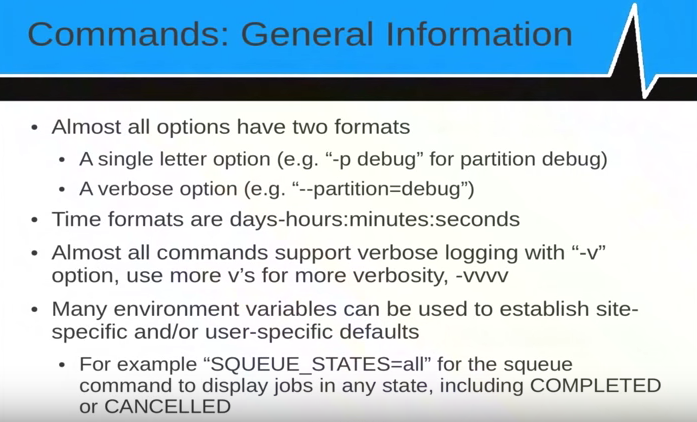
\includegraphics[width=5in]{intro-slurm-2-commands.png} 
   \caption{example caption}
%   \label{fig:example}
\end{figure}

\begin{figure}[htbp] %  figure placement: here, top, bottom, or page
   \centering
   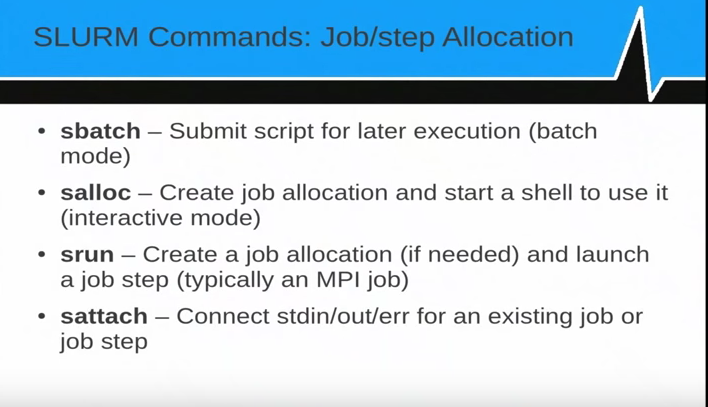
\includegraphics[width=5in]{intro-slurm-3-commands job-step.png} 
   \caption{example caption}
   %\label{fig:example}
\end{figure}

\begin{figure}[htbp] %  figure placement: here, top, bottom, or page
   \centering
   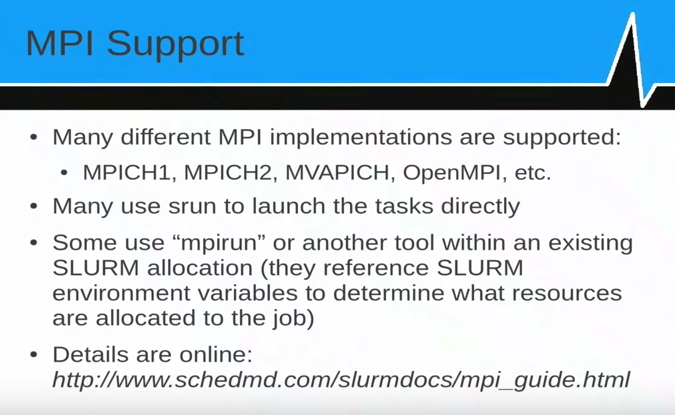
\includegraphics[width=5in]{intro-slurm-3-commands mpirun.png} 
   \caption{example caption}
   %\label{fig:example}
\end{figure}


\begin{figure}[htbp] %  figure placement: here, top, bottom, or page
   \centering
   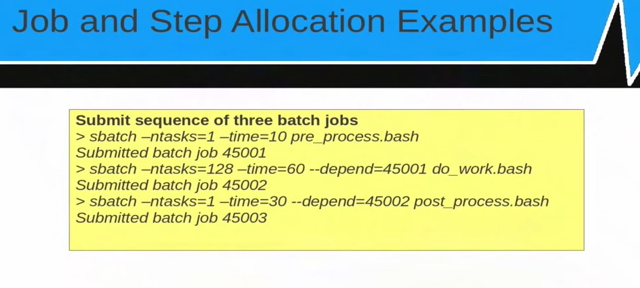
\includegraphics[width=5in]{intro-slurm-3-commands sbatch.png} 
   \caption{example caption}
   %\label{fig:example}
\end{figure}


\newpage

\begin{center}
Glossary -- from \begin{verbatim}https://www.nics.tennessee.edu/hpc-glossary\end{verbatim}
\end{center}

\begin{enumerate}
  \item
  \bigskip

\textsc{Core}

A core is an individual processor: the part of a computer which actually executes programs. CPUs used to have a single core, and the terms were interchangeable. In recent years, several cores, or processors, have been manufactured on a single CPU chip, which may be referred to as a multiprocessor. It is important to note, however, that the relationship between the cores may vary radically: AMD's Opteron, Intel's Itanium, and IBM's Cell have very distinct setups.

  
  \bigskip

  \item
  \bigskip

\textsc{CPU}

CPU stands for Central Processing Unit, and is the part of a computer which executes software programs. The term is not specific to a particular method of execution: units based on transistors, relays, or vacuum tubes might be considered CPU's. However, for clarity, we will use the term to refer to individual silicon chips, such as Intel's Pentium or AMD's Athlon. Thus, a CPU contains one or more cores, however, an HPC system may contain many CPU's. For example, Kraken contains several thousand AMD Opteron CPU's.  
  \bigskip
  
  \item
\textsc{  Node}

In traditional computing, a node is an object on a network. 

$\rightarrow$ so abstract.

For example, on a home network, your computer, router, and printer might all be nodes. 

$\rightarrow$ hmm

Supercomputers like Kraken are essentially networks, with nodes that communicate with each other to solve a larger problem than any singular computer could in a reasonable amount of time. 

$\rightarrow$ essentially networks!

Kraken contains {\color{red}several types of nodes}; {\color{blue}compute nodes} are the work-horses of the system, and are much like a stripped-down computer. An {\color{blue} I/O node} is the interface between the compute nodes and other computers, that is, it deals with input and output for the system.
  
  \bigskip

  \item
\textsc{Scratch Space}

Supercomputers generally have what is called scratch space: disk space available for temporary use. It is analogous to scratch paper. This may be thought of as a desk: it is where papers are stored while they are waiting to be worked on or filed away.

$\rightarrow$ OK. Oasis is scratch space.  One way to tell is that the letters ``temp'' are in part of Mahidhar's implementation.
  
  \bigskip

  \item
\textsc{   sbatch }- 
   
   Submit a batch script to Slurm.  Slurm = Simple Linux utility resource management.
   
   How are batch scripts different that normal, i.e. non-batch scripts?
   
   The pound sign seems to be different that a normal script, no?
  
  \bigskip

  \item
  \textsc{Slurm}
  
  Simple Linux user resource management.
  
  a man page exists on Comet
  
  http://slurm.schedmd.com/
  
  A new method of processing requests to run a program.
  
  \bigskip
  
  \bigskip
  \item
\textsc{ squeue }

to report the status of jobs

Seen many times in the history.

  \bigskip
  \item
 \textsc{daemon}
  
  In multitasking computer operating systems, a daemon (/?di?m?n/ or /?de?m?n/) is a computer program that runs as a background process, rather than being under the direct control of an interactive user.
  \bigskip
  
  \bigskip
  
  \item
  \textsc{failover}
  
``If one of the servers, or nodes, fails, another node in the cluster can take over its workload without any downtime (this process is known as failover).
''
From YouTube ``Introduction to SLURM 2''


\end{enumerate}



\end{document}  